\section{Conclusion}
Analysing the Pali canon based on average word length (AWL), corrected for abbreviations and without headers, shows that the AWL is a reliable indicator for lateness of collections and the Pali canon shows a clear trend in use of language across time. 

The clear impact of headers on the values shows that these have been added at a later date.
Verse collections as well as mātikā have a relatively lower AWL than prose of roughly the same age. 

The following graph shows the Average Word Length sorted by value and color-coded to show that early suttas have an overall lower AWL while commentaries have an overall very high AWL. It also shows that as a general trend the Vinaya, Abhidhamma and later suttas have all developed around the same time.

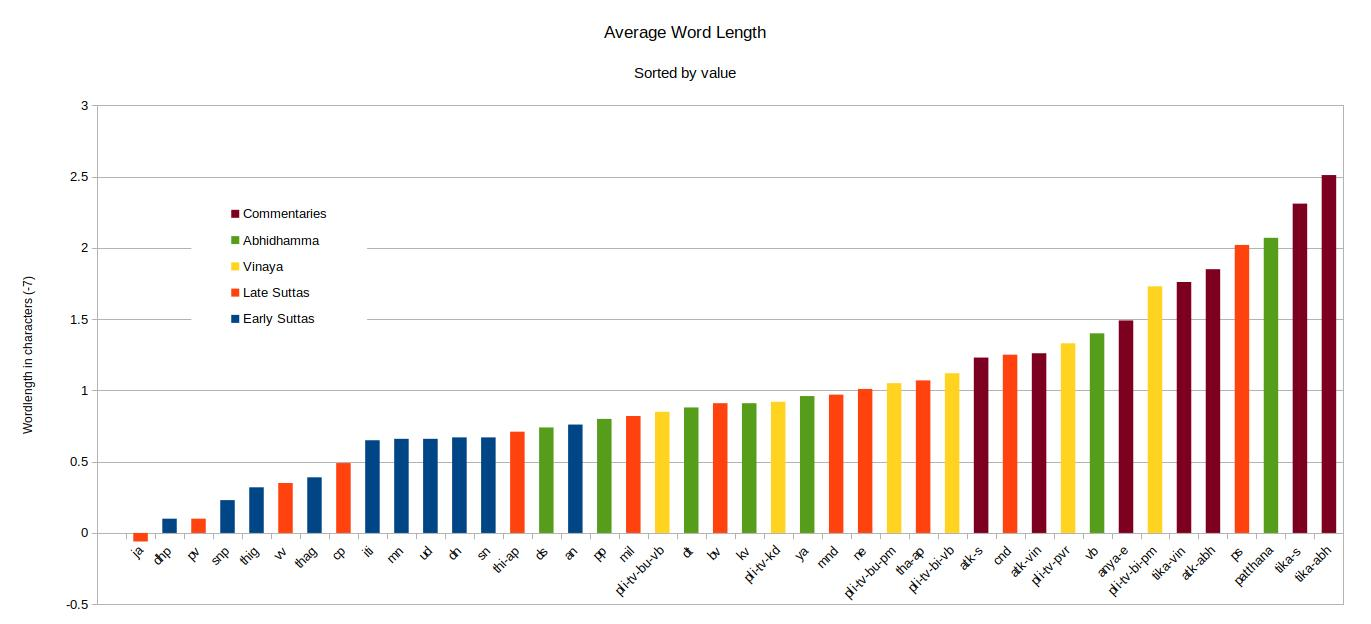
\includegraphics[width=\linewidth]{awlsorted.jpg}
\captionof{figure}{AWL sorted by value and color coded. Peṭakopadesa (pe) and Khuddakapāṭha (kp) have been omitted.}
\label{awlsorted}

\medskip
However, we have to be careful when using the AWL for files within collections because these can show considerable variations based on several factors, especially if files are very short. The AWL is only an indicator, which can be used together with other indicators like f.i. the number and quality of parallels, especially parallels with other canons from other schools. 
